\documentclass{beamer}
\usetheme[faculty=econ]{fibeamer}
\usepackage[latin1]{inputenc}
\usepackage[T1]{fontenc}
\usepackage[french]{babel}

\title[Java]{\Large{Object-Oriented Design and Programming}}
\author[C. Tibermacine]{\large{Chouki~Tibermacine}\\
  \small{Chouki.Tibermacine@umontpellier.fr}
}
%\institute{Polytech Montpellier}
\date{\tiny{IG3 2019-2020}}

\begin{document}

\begin{frame}
\titlepage
\begin{flushright}

\includegraphics[width=3.5cm]{figs/polytech.png}
\end{flushright}
\end{frame}

\begin{frame}
  \huge{Assertions \& Introduction to Java Unit Testing}
\end{frame}

\AtBeginSection[]{% Print an outline at the beginning of sections
    \begin{frame}<beamer>
      \frametitle{Outline}
%\frametitle{Outline}
      \tableofcontents[currentsection]
%      \tableofcontents
    \end{frame}}

    \begin{frame}
      \frametitle{Outline}
      \tableofcontents
    \end{frame}

\section{Assertions}
\begin{frame}
\frametitle{Design by Contract}
\begin{itemize}
\item In Java, there are several techniques for implementing \textbf{contracts} in classes:
  \begin{enumerate}
  \item with \textbf{Exceptions}: \textbf{preconditions} of methods,
    by making different if-tests (checking parameters of a method, for
    ex.)  and throwing exceptions if something is wrong
  \item with \textbf{Assertions}: \textbf{postconditions} of methods
    and \textbf{invariants}
  \end{enumerate}
\item Assertions enable to check properties in programs
\item Programs are interrupted in case an assertion is not respected
\item Assertions can be inhibited
\item They can help in debugging
\end{itemize}
\end{frame}

\begin{frame}[fragile]
  \frametitle{Assertions}
  \begin{block}{Syntax}
    \begin{lstlisting}{language=JAVA}
      assert conditionWhichMustBeTrue;
      assert conditionWhichMustBeTrue: anObject;
    \end{lstlisting}
    anObject is converted to a String and displayed
  \end{block}
  \begin{block}{Example}
    \begin{lstlisting}{language=JAVA}    
    assert (offset==sizeOfFile);
    assert (offset==sizeOfFile):
            "The file has not been parsed entirely";
    \end{lstlisting}
  \end{block}  
\end{frame}

\begin{frame}
  \frametitle{Good Practices}
  Assertions are used as:
  \begin{itemize}
  \item Invariants of an algorithm:
    \begin{itemize}
    \item At the end of an iteration to search the min value, the
      obtained value must be less than all values processed before
    \end{itemize}
  \item Stream invariants:
    \begin{itemize}
    \item This level of the program must not be reached. Example: a
      \texttt{switch-case} statement, with a \texttt{default} that
      must never be reached or a loop that must never end
    \end{itemize}
  \item Postconditions:
    \begin{itemize}
    \item After parsing a file, the offset must reach the end of
      the file
    \end{itemize}    
  \item Class invariants:
    \begin{itemize}
    \item A Person must always have an age between 0 and 140
    \end{itemize}        
  \end{itemize}
\end{frame}

\begin{frame}
  \frametitle{Bad Practices}
  Assertions must \textbf{not} be used for:
  \begin{itemize}
  \item checking the parameters of a method because they come from
    elsewhere and may be incorrect (rather, test and treat the
    problem, possibly by throwing exceptions to the caller)
  \item checking the results of interactions with a user (which can
    include errors that must be treated)
  \item creating side effects: changing the state of a program with
    assertions in the two expressions that compose them
  \end{itemize}
\end{frame}

\begin{frame}
  \frametitle{Important Notes}
  \begin{itemize}
  \item Assertions can be enabled or disabled while compiling and
    running programs
  \item By default, they are disabled
  \item Don't assume that they will be always executed
  \item Good tool when developing, testing and debugging (they enable
    to set up guards)
  \item An assertion throws an AssertionError (inherits from Error and
    then from Throwable), which must not be caught or declared to be
    thrown
  \item They are never executed in production code
  \end{itemize}
\end{frame}

\begin{frame}
  \frametitle{How to compile and run programs with assertions? with
    command-line}
  
  \begin{itemize}
  \item Compile a program by enabling assertions:\\
    \texttt{javac -source <version> MyClass.java}\\
    where \texttt{<version>} must be replaced by you JDK version
  \item Example:\\
    \texttt{javac -source 14 MyClass.java}\\
    (run \texttt{java -version} to know the version of your JDK)
  \item Run a program by enabling assertions:\\
    \texttt{java -ea MyClass}\\
    \texttt{ea} stands for ``enable assertions''
    
  \item Compile and run the program by enabling assertions:\\
    \texttt{java -ea MyClass.java}
  \end{itemize}
\end{frame}

\begin{frame}
  \frametitle{How to compile and run programs with assertions? with
    command-line}
  \begin{itemize}
  \item We can enable assertions for some packages or classes and
    disable (\texttt{-da} option) them for others
  \item Run the command:\\ \texttt{man java}\\
    then read carefully the part of the manual about -da and -ea
    options
  \end{itemize}
\end{frame}

\begin{frame}
  \frametitle{How to compile and run programs with assertions? with
    command-line}
  \begin{block}{Exercice}
    \begin{itemize}
    \item Write a class named \texttt{Say} with a
      \texttt{main(args...)}  method that prints one or several
      messages received as argument(s) (in \texttt{args} array).
  \item Put an assertion that checks if at least one argument is
    received by this method
  \item Compile and run your program with and without arguments and options:\\
  \texttt{java Say}\\
  \texttt{java -ea Say}\\
  \texttt{java -ea Say "Hello World!"}
  \end{itemize}
  \end{block}
\end{frame}

\begin{frame}
  \frametitle{How to compile and run programs with assertions? In IDEs}
    \begin{tikzpicture}[overlay,remember picture]
    \node[anchor=center,xshift=0pt,yshift=-35pt]
    at (current page.center) {
      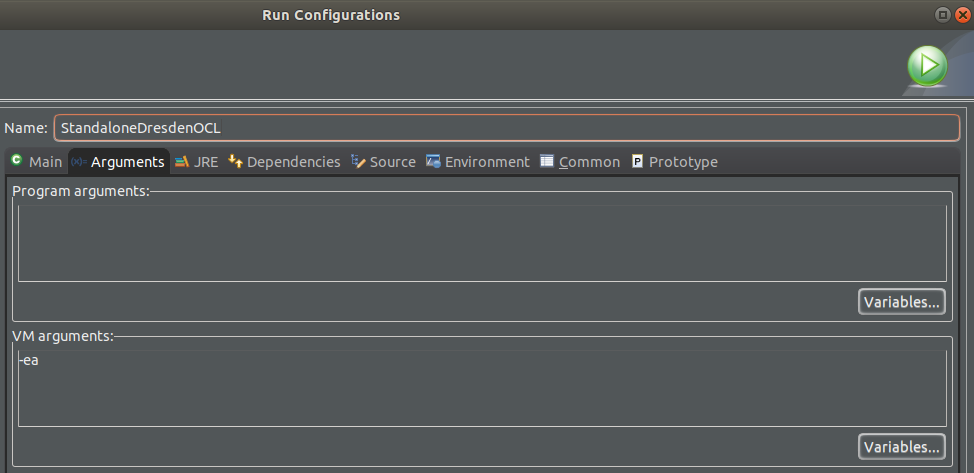
\includegraphics[width=10cm]{img/eclipse_assertions.png}
    };
  \end{tikzpicture}
  \begin{itemize}
  \item In Eclipse, Menu Run then Run Configurations (see Figure)
    \vspace{5cm}
  \item Tell us on Slack how to do it in your favorite IDE
\end{itemize}
\end{frame}

\section{Automatic Unit Testing in Java}

\subsection{Introduction}

\begin{frame}
\frametitle{Why to Automate Tests?}
\begin{itemize}
\item Identify problems in the code the earliest possible and fix them
  before it becomes too expensive to fix them
\item Repeat them in time
\item More generally:
  \begin{itemize}
  \item Achieve stakeholders goals
  \item Meet functional requirements
  \item Correctly handle corner/edge cases
  \item \textbf{Continuously deliver reliable code}
  \item \textbf{Remove fear from change}
  \end{itemize}    
\end{itemize}
\end{frame}

\begin{frame}
\frametitle{Testing Hierarchy}
\begin{itemize}
\item Three types of tests, from most specific (and simplest) to most general (and most complex):
  \begin{enumerate}
  \item Unit Tests (object of this course)
  \item Aggregation/Integration Tests (test components of the system)
  \item System Tests (end-to-end tests)
  \end{enumerate}
\item Unit testing: test a single unit of functionality (a method, a
  class, or a small module), \textbf{a single unit of behavior}
\end{itemize}
\end{frame}

\begin{frame}
\frametitle{A Tool for writing and executing Tests: JUnit}
\begin{itemize}
\item Origins: Xtreme Programming (Test-First Development) and Agile Methods
\item Test Framework written in Java by E. Gamma and K. Beck
\item Open Source Project: \url{http://www.junit.org}
\item There are other frameworks, but this is the most popular one
\end{itemize}
\end{frame}

\subsection{Testing Code}
\begin{frame}
\frametitle{A First Example (from R. Warburton)}
\begin{itemize}
\item Let us write an app which represents a Cafe that stores beans
  and milk and enables to brew coffee to produce different kinds of
  coffees
\item 3 classes:
  \begin{itemize}
  \item CoffeeType: Enum of different kinds of Coffee
  \item Coffee: a class for a single cup of coffee
  \item Cafe: a class for brewing coffee
  \end{itemize}    
\end{itemize}
\end{frame}

\begin{frame}
\frametitle{A First Example: Coffee class}
    \begin{tikzpicture}[overlay,remember picture]
    \node[anchor=center,xshift=0pt,yshift=-20pt]
    at (current page.center) {
      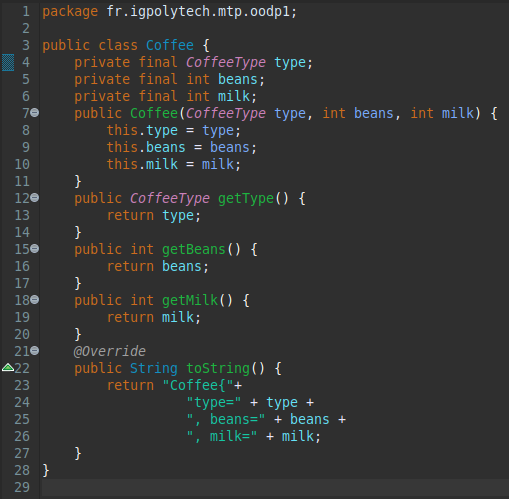
\includegraphics[width=8cm]{img/Coffee.png}
    };
  \end{tikzpicture}
\end{frame}

\begin{frame}
\frametitle{A First Example: Cafe class}
    \begin{tikzpicture}[overlay,remember picture]
    \node[anchor=center,xshift=0pt,yshift=-20pt]
    at (current page.center) {
      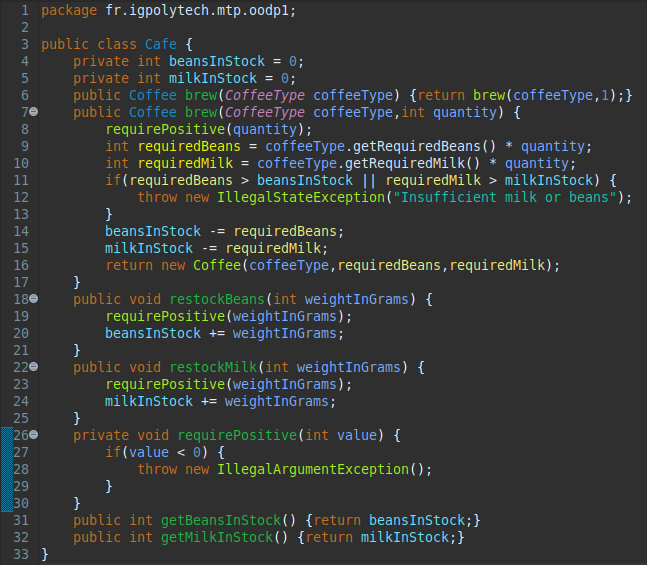
\includegraphics[width=9cm]{img/Cafe.png}
    };
  \end{tikzpicture}
\end{frame}

\begin{frame}
\frametitle{A First Example: CoffeeType enum}
    \begin{tikzpicture}[overlay,remember picture]
    \node[anchor=center,xshift=0pt,yshift=-5pt]
    at (current page.center) {
      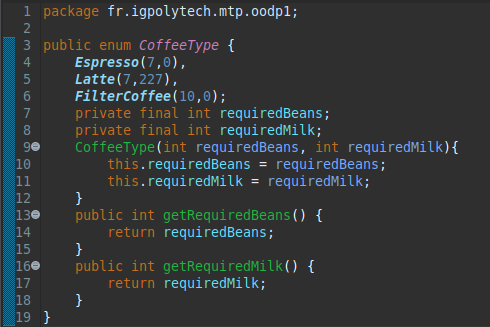
\includegraphics[width=9cm]{img/CoffeeType.png}
    };
  \end{tikzpicture}
  \begin{itemize}
  \vspace{5cm}
\item[] The code is available on Moodle
  \end{itemize}
\end{frame}

\begin{frame}
\frametitle{Testing the Cafe class}
\begin{itemize}
\item The main functionality to test is associated to brew method
\item In Java, by convention, for a given class we write a Testing
  class: a \texttt{CafeTest} class in our example
\item In the testing class, we write a series of methods each of which
  corresponds to a behavior (each method is a \textbf{Test Case}):
  \begin{itemize}
  \item can we brew some Espresso?
  \item ...
  \end{itemize}
\item Each method should have a name that corresponds to the test made
  (don't use testBrew1, testBrew2, ...)
\item In JUnit, methods must be annotated \texttt{@Test} so that the
  framework will invoke them in a certain way
\end{itemize}
\end{frame}

\begin{frame}
\frametitle{A First Test Example: CafeTest class}
    \begin{tikzpicture}[overlay,remember picture]
    \node[anchor=center,xshift=0pt,yshift=-5pt]
    at (current page.center) {
      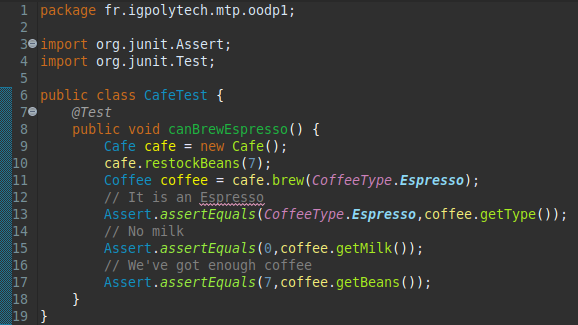
\includegraphics[width=10cm]{img/CafeTest.png}
    };
  \end{tikzpicture}
  \vspace{5.2cm}
\begin{itemize}
\item[]  Plenty of assertions: \texttt{assertTrue(...)},
  \texttt{assertFalse(...)}, \texttt{assertNull(...)},
  \texttt{assertSame(...)}, ...
  \end{itemize}
\end{frame}

\begin{frame}
\frametitle{A First Test Example: Running the Test}
    \begin{tikzpicture}[overlay,remember picture]
    \node[anchor=center,xshift=0pt,yshift=-20pt]
    at (current page.center) {
      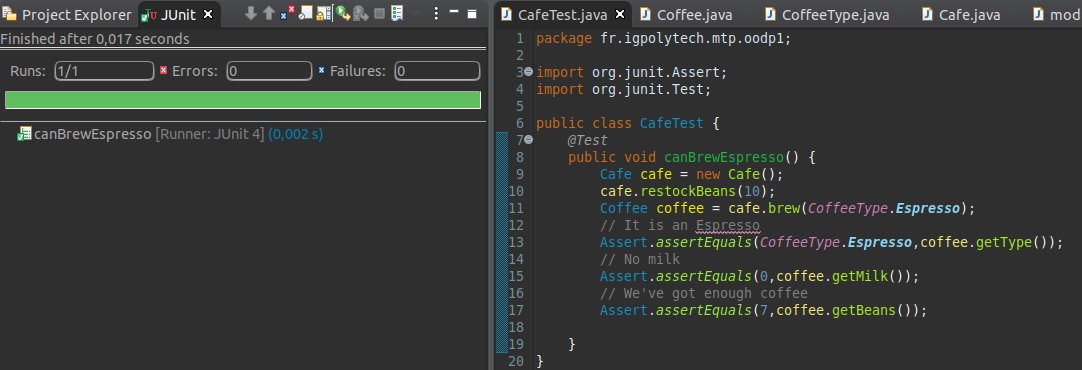
\includegraphics[width=12cm]{img/CafeTestRun.png}
    };
  \end{tikzpicture}
  \begin{itemize}
  \item On Eclipse, right-click on the method
    \texttt{canBrewEspresso()}, then choose menu item ``\texttt{Run
      As}'', and at last ``\texttt{JUnit Test}'' \vspace{4.2cm}
  \item Try it and try to break the tests. What happens?
  \item Did you notice that we do not invoke test methods? JUnit do it
    \footnotesize
  \item Don't forget to add JUnit Library in
    the build-path of your IDE Project
    \normalsize
  \end{itemize}
  
\end{frame}

\begin{frame}
\frametitle{Test Results}

  \begin{itemize}
  \item Pass/Run (green): no errors and failures
  \item Errors (red): tests do not run properly    
  \item Failures (red): tests run properly but the tested behavior does
    not execute properly
  \end{itemize}
  
\end{frame}

\begin{frame}
\frametitle{A First Test Example: Running the Test with Failure}
    \begin{tikzpicture}[overlay,remember picture]
    \node[anchor=center,xshift=0pt,yshift=-30pt]
    at (current page.center) {
      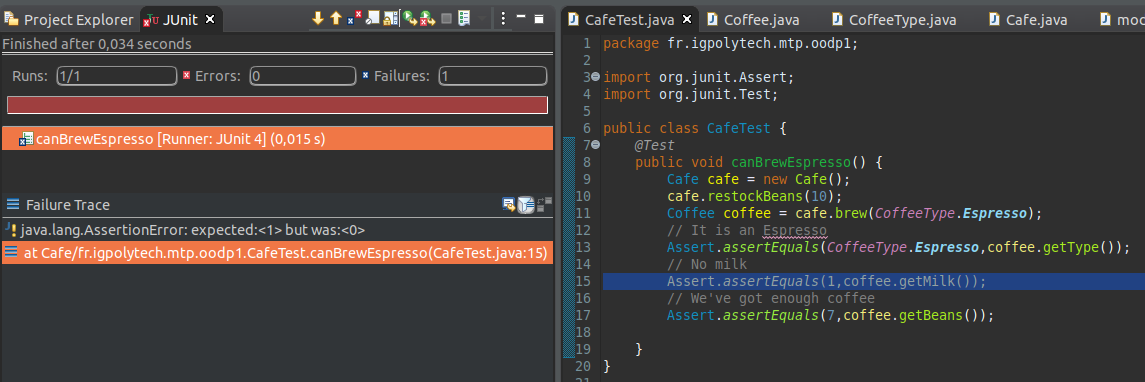
\includegraphics[width=12cm]{img/CafeTestRunFailure.png}
    };
  \end{tikzpicture}
  \begin{itemize}
  \item After having changed Line 15 (replaced 0 by 1) \vspace{4.5cm}
  \item See the view at the left. What is in there?
  \end{itemize}  
\end{frame}

\begin{frame}
\frametitle{Running Tests with Command Line}
\begin{itemize}
\item This is possible, but we need to solve many dependencies (a
  cumbersome task when done manually)
\item This is made easy by the well-known \textbf{Build Tools} like
  Maven or Gradle
\item Next year, we'll have a course on these tools, and you'll see
  how it is easy to work on large Java projects with multiple
  dependencies and many build steps (download dependencies like JUnit,
  compile, test, build JAR, generate documentation, ...)
\end{itemize}
\end{frame}

\begin{frame}
  \frametitle{Common Structure for Tests}
  Three clauses in a Test:
\begin{itemize}
\item \textbf{Given} clause: What should the world looks like when the
  behavior happens? (the preconditions)
\item \textbf{When} clause: What is being tested? (a simple isolated
  behavior)
\item \textbf{Then} clause: What are the changes that happened? (the
  postcondition)
\end{itemize}
\end{frame}

\begin{frame}
  \frametitle{Common Structure for Tests on our Example}
  \begin{tikzpicture}[overlay,remember picture]
    \node[anchor=center,xshift=0pt,yshift=0pt]
    at (current page.center) {
      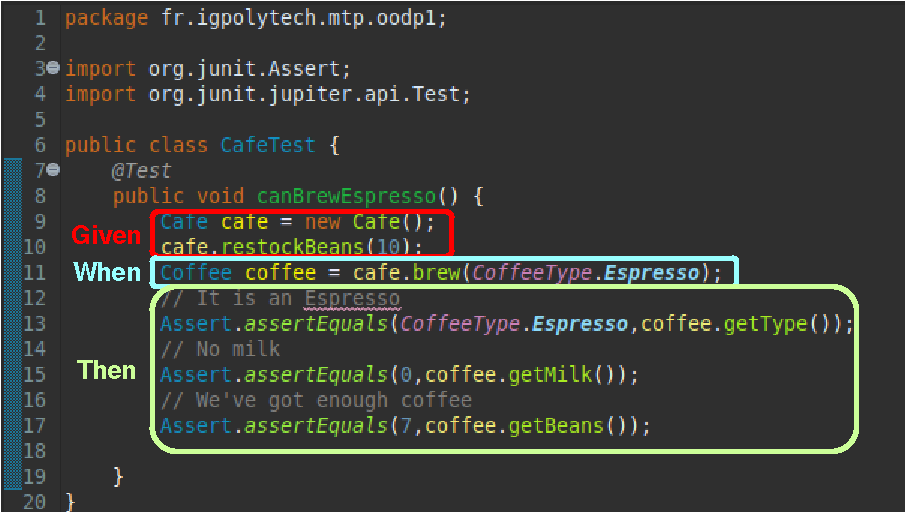
\includegraphics[width=10cm]{img/tests_structure.pdf}
    };
  \end{tikzpicture}
\end{frame}

\begin{frame}
\frametitle{Exercice}
\begin{itemize}
\item Write a second test method for ensuring that brewing espresso
  consumes beans in the stock
\item The same \texttt{Given} and \texttt{When} clauses
\end{itemize}
\end{frame}

\begin{frame}[fragile]
  \frametitle{Exceptions, Failures and Errors}
  % \begin{tikzpicture}[overlay,remember picture]
  %   \node[anchor=south,xshift=0pt,yshift=10pt]
  %   at (current page.south) {
  %     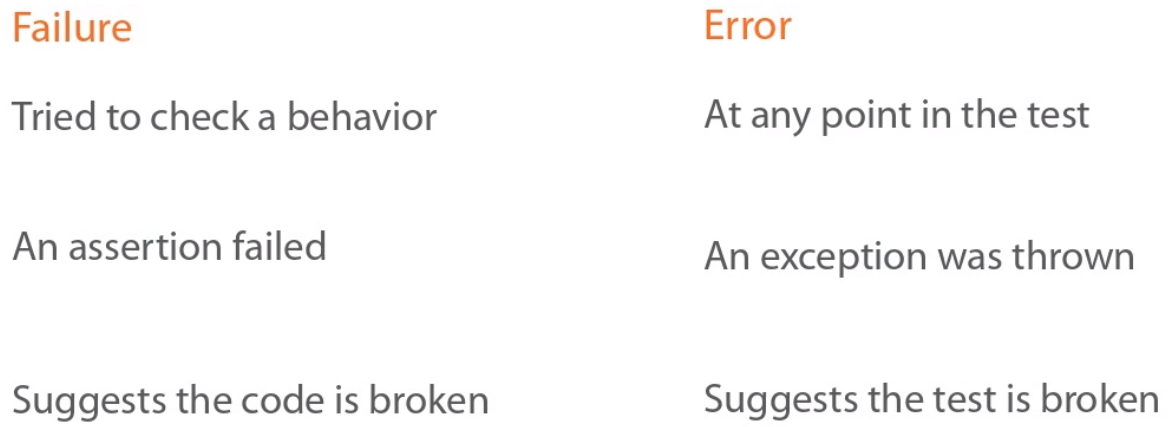
\includegraphics[width=10cm]{img/failures_vs_errors.png}
  %   };
  % \end{tikzpicture}
\begin{itemize}
\item Sometimes an exception is the correct result (a wrong input from
  a user)
\item If we want to check the throwing of the exception in the code:
\begin{lstlisting}[language=JAVA]
// Then clause    
@Test(expected=IllegalArgumentException.class)
public void lattesRequireMilk() {
  // Given clause
  Cafe cafe = new Cafe();
  cafe.restockBeans(7);
  // When clause
  cafe.brew(CoffeeType.Latte);
}
\end{lstlisting}
\item[] Without the parameter of the \texttt{@Test} annotation, we'll
  get a failure. Why? \only<2>{{\color{red}Because the When clause
      produces an exception which is not handled}}
\end{itemize}
\end{frame}

\begin{frame}[fragile]
  \frametitle{Exceptions, Failures and Errors -- Ctd}
  \begin{tikzpicture}[overlay,remember picture]
    \node[anchor=south,xshift=20pt,yshift=20pt]
    at (current page.south) {
      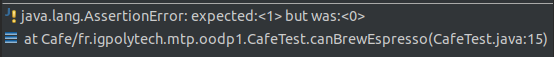
\includegraphics[width=8cm]{img/AssertionError.png}
    };
  \end{tikzpicture}
  \begin{itemize}
  \item Failures vs Errors:
    \begin{itemize}
    \item An error: a problem with the code of the test (must be
      fixed so that the test checks the behavior properly)
    \item A failure: the test runs correctly but the tested code does not
      provide the expected behavior
      \begin{itemize}
      \item It is what we get when we tried to break the tests in the
        previous example (replacing 0 by 1 in the second Then clause)
      \item The assertions executed by JUnit throw an
        \texttt{AssertionError} with details about the test (expected
        and actual values)
      \end{itemize}
    \end{itemize}
  \end{itemize}
\end{frame}

\subsection{Writing Good Tests}
\begin{frame}
\frametitle{Good Practices}
\begin{itemize}
\item Give good names to tests: important for readability and thereby
  help in maintenance/evolution
  \begin{itemize}
  \item Be descriptive: the name should reflect when and then clauses,
    even if it is a too long name
  \item Use app domain terminology and natural language in naming
  \end{itemize}
\item Test the behavior not the implementation
\item DRY: Don't Repeat Yourself (avoid duplication when writing tests)
\item Diagnostics (output) should help in identifying the problem to fix
\end{itemize}
\end{frame}

\begin{frame}
\frametitle{Behavior Not Implementation}
\begin{itemize}
\item Test only the public API (public methods of a class)
\item Do not trespassing private members of a class
\item Do not expose private members to test them  
\item Even if we change the implementation of a tested method (use a
  different data structure, for example), the test should continue to
  run properly
\item Test cases should be independent the ones from the others
\item Tests cases are defined without parameters and have
  \texttt{void} as a return type
\end{itemize}
\end{frame}

\begin{frame}
\frametitle{DRY: Don't Repeat Yourself}
\begin{itemize}
\item In our previous two test cases, the Given and When clauses are
  repeated. This is an anti-pattern (\textit{Duplication
    Anti-pattern})
\item This produces several places to change
\item These two clauses should be put in a single place
  \begin{itemize}
  \item  Do it in your copy of the code
  \end{itemize}
\item The value 7 used in the Given clause should be replaced by a
  constant (\texttt{ESPRESSO\_BEANS}). The same for value 0
  (\texttt{NO\_MILK} constant). This is more readable and prevents
  duplication of these values
\end{itemize}
\end{frame}

\begin{frame}[fragile]
\frametitle{Diagnostics}
\begin{itemize}
\item If we want to compare values in a test, we have to expose
  values, by privileging \texttt{assertEquals(...)} to
  \texttt{assertTrue()}
\item The latter assertion produces only an assertion error. Example
\begin{lstlisting}[language=JAVA]
assertTrue(aList.size() == 1);
// Should be replaced by:
assertEquals(1,aList.size());
// This will print: expected value=1, but the actual value=0
// for example in a failing test
// We can go further by writing
assertEquals("Wrong quantity of coffee",1,aList.size());
\end{lstlisting}
\item Go back to our example and add String messages like above
\end{itemize}
\end{frame}

\begin{frame}
\frametitle{Before and after tests}
\begin{itemize}
\item JUnit provides annotations that can be used for indicating code parts that must be executed before and after test running
\item Annotations used for methods:
  \begin{itemize}
  \item \texttt{@Before}: Before each test method runs 
  \item \texttt{@After}: After each test method runs
  \item \texttt{@BeforeClass}: Before all tests in the class (used to
    annotate static methods)
  \item \texttt{@AfterClass}: After all tests in the class (used to
    annotate static methods)
  \end{itemize}
\item Use the \texttt{@Before} annotation to annotate a method that
  you have to write and which contains the creation of the object
  \texttt{Cafe} needed in each test (change the test cases)
\item \texttt{@Test} annotation can have a \texttt{timeout} parameter:\\
  \texttt{@Test(timeout=10)}\\
  The test fails if the test executes in more than 10ms
\end{itemize}
\end{frame}

\begin{frame}[fragile]
\frametitle{Testing with JUnit 5}
\begin{itemize}
\item Assertion methods (\texttt{assertEquals(...)}, ...) are provided
  by class \texttt{Assertions} from \texttt{org.junit.jupiter.api}
\begin{tiny}
\begin{lstlisting}[language=JAVA]
import org.junit.jupiter.api.Assertions;
...
Assertions.assertEquals(...)

// or a static import of all methods from Assertions:
import static org.junit.jupiter.api.Assertions.*;
...
assertEquals(...)
\end{lstlisting}                
\end{tiny}
\item \texttt{@Before} $\rightarrow$ \texttt{@BeforeEach}, ...
\item More details in:
  \footnotesize
  \url{https://junit.org/junit5/docs/current/api/}
  \normalsize
\end{itemize}
\end{frame}

\begin{frame}[fragile]
\frametitle{AssertThat (since JUnit 4.4)}
\begin{itemize}
  \item \texttt{assertThat([value], [matcher statement]);}
  \item Examples :
\begin{itemize}
  \item assertThat(x, is(3));
  \item assertThat(x, is(not(4)));
  \item assertThat(responseString, either(containsString("color")).or(containsString("colour")));
\item assertThat(myList, hasItem("3"));
\end{itemize}
  \item not(s), either(s).or(ss), each(s)
\item Diagnostic messages are more clear
\item Use \texttt{org.hamcrest.MatcherAssert.assertThat(...)} instead of
  \texttt{Assert.assertThat(...)} (the latter is deprecated)
\item All (static) methods is(), not(), ... can be imported statically:
\begin{lstlisting}[language=JAVA]
import static org.hamcrest.CoreMatchers.*;
\end{lstlisting}  
\end{itemize}
\end{frame}

\subsection{Parameterized Tests and Test Suites}
%--------------------------------------------------------
\begin{frame}
\frametitle{Parameterized Test}
\begin{itemize}
  \item Goal: reuse a test method (case) with different datasets
  \item Test datasets:
\begin{itemize}
\item returned by a method annotated \texttt{@Parameters}
\item This method returns a collection of arrays containing the data
  and possibly the expected result
\end{itemize}
  \item Test Class:
\begin{itemize}
  \item annotated @RunWith(Parameterized.class)
  \item contains methods which must be executed with each dataset
\end{itemize}
\item For each data, the class is instantiated and the test methods
  are executed
\end{itemize}
\end{frame}
%--------------------------------------------------------
\begin{frame}
\frametitle{Parameterized Tests: the Requirements}
\begin{itemize}
\item A Public constructor which uses the parameters (the dataset)
  
  \item The method which returns the parameters (datasets) must be static
\end{itemize}
\end{frame}
%--------------------------------------------------------
\begin{frame}[fragile]
\frametitle{Example of a Parameterized Test -- to be tested}
\begin{tiny}\begin{lstlisting}[language=JAVA]
import org.junit.Test; import org.junit.runner.RunWith;
import org.junit.runners.Parameterized;
import org.junit.runners.Parameterized.Parameters;
import static org.junit.Assert.*; import java.util.*;
@RunWith(Parameterized.class)
public class TestParamSum {
  private int x; private int y; private int res;
  public TestParamSum(int x, int y, int res) {
    this.x = x; this.y = y; this.res = res;}
  @Parameters
  public static Collection testData() {
  return Arrays.asList(new Object[][] {
    { 0, 0, 0 },{ 1, 1, 2 },{ 2, 1, 3 },{10, 9, 19}});}
  @Test
  public void sumCalculatesAddition() {
    assertEquals(res,new Sum().sum(x,y)); }
}
\end{lstlisting}
\end{tiny}
\end{frame}

\begin{frame}[fragile]
\frametitle{Test Suites}
\begin{itemize}
  \item Group test cases in order to chain their execution
  \item i.e. group the execution of test classes
  \item Example: -- to be tested (by replacing TestClass1 and
    TestClass2 by the previous two classes, CafeTest and TestParamSum)
\end{itemize}
\begin{tiny}
\begin{lstlisting}[language=JAVA]
import org.junit.runner.RunWith;
import org.junit.runners.Suite;
@RunWith(Suite.class)
@Suite.SuiteClasses({
        TestClass1.class,
        TestClass2.class
        })
public class MyTestSuite {
}
\end{lstlisting}                
\end{tiny}

\end{frame}

\begin{frame}

      \begin{tikzpicture}[overlay,remember picture]
        \node[anchor=center,xshift=0pt,yshift=0pt]
        at (current page.center) {
          
\includegraphics[width=4cm]{img/question.jpg}
        };
      \end{tikzpicture}

\end{frame}

\end{document}
